\documentclass[tikz,border=8pt]{standalone}
\usepackage[T1]{fontenc}
\usepackage{helvet}
\renewcommand{\familydefault}{\sfdefault}
\usepackage{graphicx}
\usepackage{xcolor}
\usepackage{tikz}
\usetikzlibrary{arrows.meta,backgrounds,calc,fit,positioning,shapes.geometric}

\definecolor{sgnavy}{HTML}{173B72}
\definecolor{sgblue}{HTML}{2E6DB4}
\definecolor{sgteal}{HTML}{25A7A1}
\definecolor{sgred}{HTML}{E63B47}
\definecolor{sgorange}{HTML}{F28C28}
\definecolor{sggreen}{HTML}{4D9460}
\definecolor{sggray}{HTML}{5F6B76}
\definecolor{sglight}{HTML}{F2F5F8}
\definecolor{sgline}{HTML}{CBD5DF}

\tikzset{
  box/.style={
    draw=sgline,
    fill=white,
    rounded corners=2pt,
    line width=.7pt,
    minimum height=13mm,
    text width=28mm,
    align=center,
    inner sep=3mm,
    font=\small
  },
  compactbox/.style={
    draw=sgline,
    fill=white,
    rounded corners=2pt,
    line width=.7pt,
    minimum height=10mm,
    text width=23mm,
    align=center,
    inner sep=2mm,
    font=\scriptsize
  },
  sourcebox/.style={
    box,
    draw=sgblue,
    fill=sgblue!5
  },
  servicebox/.style={
    box,
    draw=sgteal,
    fill=sgteal!5
  },
  databox/.style={
    box,
    draw=sggreen,
    fill=sggreen!6
  },
  decisionbox/.style={
    diamond,
    draw=sgnavy,
    fill=white,
    aspect=2.4,
    align=center,
    inner sep=1.8mm,
    font=\scriptsize
  },
  layerbox/.style={
    draw=sgline,
    fill=sglight,
    rounded corners=3pt,
    inner sep=5mm
  },
  flow/.style={
    -{Latex[length=2.5mm]},
    line width=1pt,
    draw=sgnavy
  },
  dataflow/.style={
    -{Latex[length=2.5mm]},
    line width=1pt,
    draw=sgteal
  },
  warningflow/.style={
    -{Latex[length=2.5mm]},
    line width=1pt,
    draw=sgred
  },
  labeltext/.style={font=\scriptsize, text=sggray, align=center, fill=white, inner sep=1.5pt},
  zonelabel/.style={font=\bfseries\scriptsize, text=sgnavy, fill=sglight, inner sep=1pt},
  titletext/.style={font=\bfseries\large, text=sgnavy}
}

\begin{document}
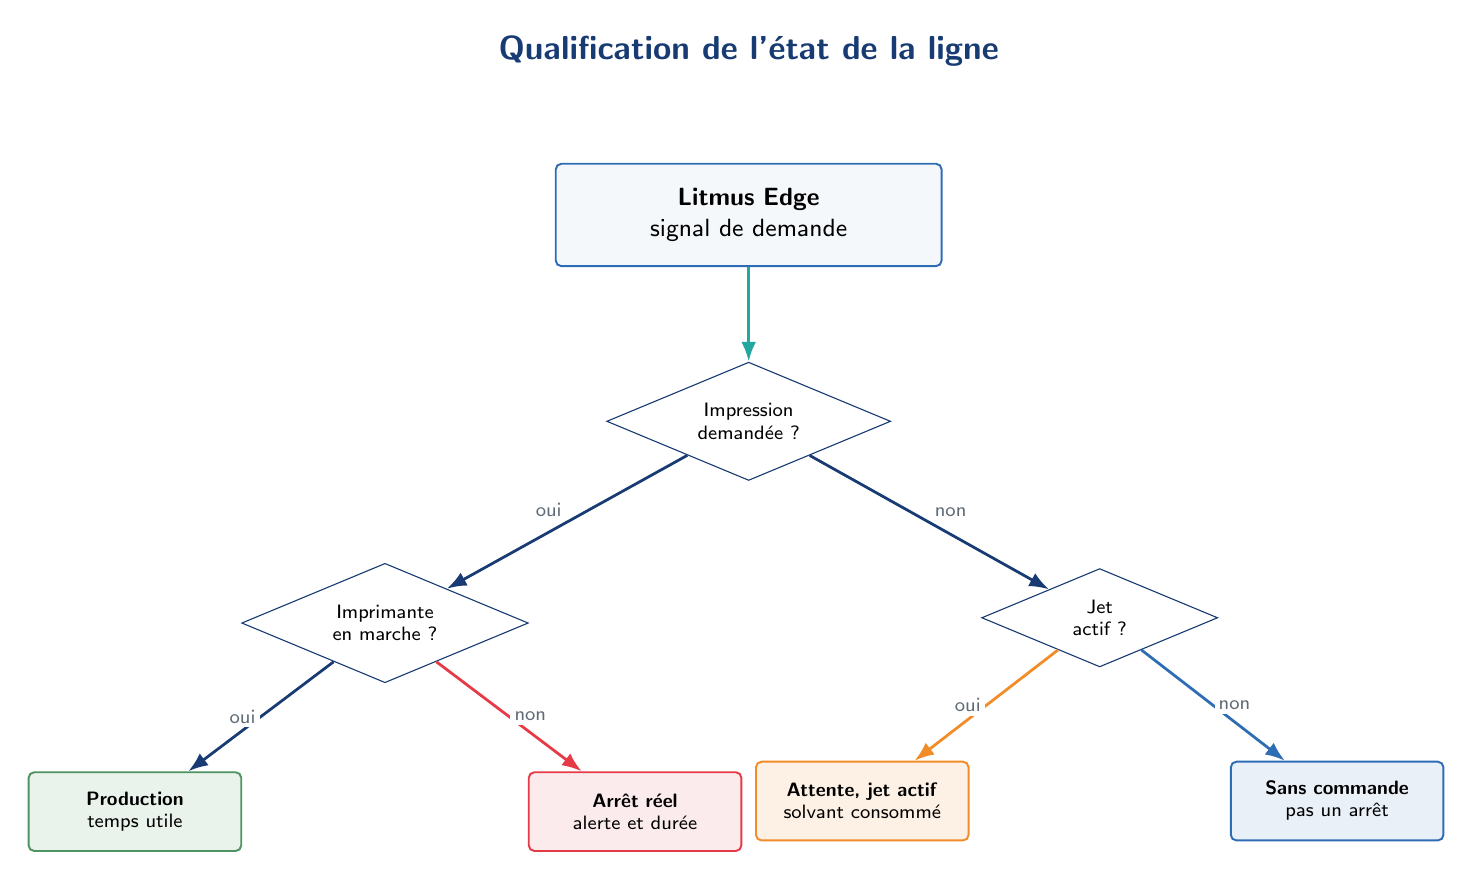
\begin{tikzpicture}[node distance=8mm]
  \node[titletext] (title) {Qualification de l'état de la ligne};
  \node[sourcebox, below=11mm of title, text width=43mm] (litmus)
    {\textbf{Litmus Edge}\\signal de demande};
  \node[decisionbox, below=12mm of litmus] (demand)
    {Impression\\demandée ?};
  \draw[dataflow] (litmus) -- (demand);

  \node[decisionbox, below left=18mm and 28mm of demand] (runningyes)
    {Imprimante\\en marche ?};
  \node[decisionbox, below right=18mm and 28mm of demand] (runningno)
    {Jet\\actif ?};
  \draw[flow] (demand) -- node[labeltext, above left]{oui} (runningyes);
  \draw[flow] (demand) -- node[labeltext, above right]{non} (runningno);

  \node[compactbox, below left=15mm and 9mm of runningyes,
        fill=sggreen!12, draw=sggreen] (prod)
    {\textbf{Production}\\temps utile};
  \node[compactbox, below right=15mm and 9mm of runningyes,
        fill=sgred!10, draw=sgred] (down)
    {\textbf{Arrêt réel}\\alerte et durée};
  \node[compactbox, below left=15mm and 9mm of runningno,
        fill=sgorange!12, draw=sgorange] (idlejet)
    {\textbf{Attente, jet actif}\\solvant consommé};
  \node[compactbox, below right=15mm and 9mm of runningno,
        fill=sgblue!10, draw=sgblue] (idle)
    {\textbf{Sans commande}\\pas un arrêt};

  \draw[flow] (runningyes) -- node[labeltext, left]{oui} (prod);
  \draw[warningflow] (runningyes) -- node[labeltext, right]{non} (down);
  \draw[flow, draw=sgorange] (runningno) -- node[labeltext, left]{oui} (idlejet);
  \draw[flow, draw=sgblue] (runningno) -- node[labeltext, right]{non} (idle);
\end{tikzpicture}
\end{document}
